
\newpage
\section{Michał Duda}
\label{sec:dudmich}


\begin{CJK}{UTF8}{min}

\subsection{日本国憲法第9条}
日本国憲法第9条は日本国憲法の一番議論の条文ということです。

\begin{framed}
\textbf{第二章 戦争の放棄}\\
第九条 日本国民は、正義と秩序を基調とする国際平和を誠実に希求し、国権の発動たる戦争と、武力による威嚇又は武力の行使は、国際紛争を解決する手段としては、永久にこれを放棄する。\\
前項の目的を達するため、陸海空軍その他の戦力は、これを保持しない。国の交戦権は、これを認めない。
\end{framed}

公的な英語の翻訳:

\begin{framed}
\textbf{RENUNCIATION OF WAR Article 9.}\\
Aspiring sincerely to an international peace based on justice and order, the Japanese people forever renounce war as a sovereign right of the nation and the threat or use of force as means of settling international disputes.\\
In order to accomplish the aim of the preceding paragraph, land, sea, and air forces, as well as other war potential, will never be maintained. The right of belligerency of the state will not be recognized.
\end{framed}

議論的といえば、日本国憲法第9条に日本は自衛権があるかどうか何も書いてありません。そのために昭和29年(1954年)に自衛隊《略称: JSDF》は、日本の独立を守り、国の安全を保つために設置されました。自衛隊は国際連合を支えて、湾岸戦争に1991年の武力介入ときから、どこまで日本自衛権が届くかの議論があっています。
\end{CJK}

\newpage
\subsection{FIAT Panda - la grande utilitaria}
Mały wielki \textit{Fiat Panda} pierwszej generacji (tipo 141A) zadebiutował w roku 1980 i bardzo szybko podbił serca Europejczyków. W ciągu 23 lat sprzedano niemalże 4.5 miliona egzemplarzy (nie licząc egzemplarzy sprzedanych przez Seata na licencji Fiata). Jego popularność nie powinna dziwić - Fiat Panda jest takim samochodem, jakim idealny samochód być powinien. Napędzany był bardzo różnorodnymi jednostkami silnikowymi (wśród nich jeden wolnossący diesel 1.3), każda z nich zapewniała doskonałą dynamikę jazdy. Legendarna jednostka 1000 FIRE była wyjątkowa w swojej prostocie i bezawaryjności. Mały miś z takim silnikiem idealnie odnajduje się nawet w dzisiejszym ruchu (co sam mogę dumnie potwierdzić!). Tabela \ref{tab:silniki_panda} przedstawia wybrane parametry niektórych jednostek silnikowych oferowanych we Fiacie Panda 141A.\\
\begin{table}[h]
\centering
\resizebox{\textwidth}{!}{%
\begin{tabular}{|c|c|c|c|c|}
\hline
\textbf{Model} &
  \textbf{\begin{tabular}[c]{@{}c@{}}Pojemność skokowa\\ \((cm^3)\)\end{tabular}} &
  \textbf{\begin{tabular}[c]{@{}c@{}}Moc\\ \((KM)\)\end{tabular}} &
  \textbf{\begin{tabular}[c]{@{}c@{}}Prędkość maksymalna\\ \((km/h)\)\end{tabular}} &
  \textbf{\begin{tabular}[c]{@{}c@{}}Konsumpcja paliwa\\ \((km/l)\)\end{tabular}} \\ \hline
\textbf{34}            & 652  & 34 & 117 & 15.6 \\ \hline
\textbf{45}            & 903  & 45 & 140 & 13.8 \\ \hline
\textbf{4x4}           & 965  & 48 & 133 & 13.8 \\ \hline
\textbf{750 Young}     & 769  & 34 & 127 & 17.5 \\ \hline
\textbf{750 FIRE}      & 769  & 39 & 125 & 18.5 \\ \hline
\textbf{900 i.e. cat.} & 899  & 39 & 135 & 18.5 \\ \hline
\textbf{900 Dance}     & 903  & 45 & 135 & 15   \\ \hline
\textbf{1000}          & 999  & 45 & 140 & 15   \\ \hline
\textbf{1000 FIRE}     & 999  & 45 & 140 & 16.1 \\ \hline
\textbf{1000 4x4}      & 999  & 50 & 136 & 14   \\ \hline
\textbf{1100 FIRE}     & 1108 & 54 & 140 & 15   \\ \hline
\textbf{1300 Diesel}   & 1301 & 37 & 130 & 18   \\ \hline
\end{tabular}%
}
\caption{Wybrane parametry niektórych silników dostępnych we Fiacie Panda pierwszej generacji (Tipo 141A)}
\label{tab:silniki_panda}
\end{table}\\

Fiat Panda 141A naturalnie przychodził z bogatym wyposażeniem, które w standardzie obejmowało:
\begin{itemize}
    \item kierownicę,
    \item przednią szybę,
    \item opony.
\end{itemize}

Wspomniałem wcześniej, że Fiat Panda był takim samochodem, jakim samochód był powinien. Pod wieloma aspektami jest lepszy niż samochody współczesne. Jestem w stanie to udowodnić następującymi argumentami:
\begin{enumerate}
    \item jeśli w trakcie jazdy prosto obrócisz kierownicę delikatnie w lewo, to samochód zjedzie ze swojego pasa w lewo. We współczesnych samochodach to nie przejdzie - zaczną piszczeć, bo "zjeżdżasz ze swojego pasa", a kierownica będzie wibrować. Może nawet samochód zacznie z tobą walczyć próbując wyrównać tor jazdy. Panda 1:0 nowe auta
    \item Liczne wersje kolorystyczne i specjalne. Panda Pink była różowa, Panda Dance miała niebiesko-fioletowe fotele, Panda Cafe miała beżowe wnętrze, Panda Verde była cała zielona (nawet silnik!), Panda College miała tapicerki w kratę, Panda Elegansa była czarna z czerwonym wnętrzem... Współcześnie samochody występują głównie w trzech kolorach: biały, szary i czarny. Panda 2:0 nowe auta
    \item niesamowita widoczność z miejsca kierowcy, obecnie w większości małych samochodów szyby są niesamowicie małe i ciemne. Panda 3:0 nowe auta. Miś wygrywa!
\end{enumerate}

Kupując Pandę można było także dobrać wiele opcji dodatkowego luksusowego wyposażenia, między innymi:
\begin{itemize}
    \item podgrzewana tylna szyba,
    \item prawe lusterko,
    \item pasy bezpieczeństwa z tyłu,
    \item uchylne szyby tylne,
    \item światła awaryjne,
    \item radio.
\end{itemize}

Zdjęcie \ref{fig:Panda_esterni} przedstawia Fiata Pandę 141A z pierwszych 5 lat produkcji, a na zdjęciu \ref{fig:Panda_interni} przedstawiono wnętrze z późniejszych lat.

\begin{figure}[H]
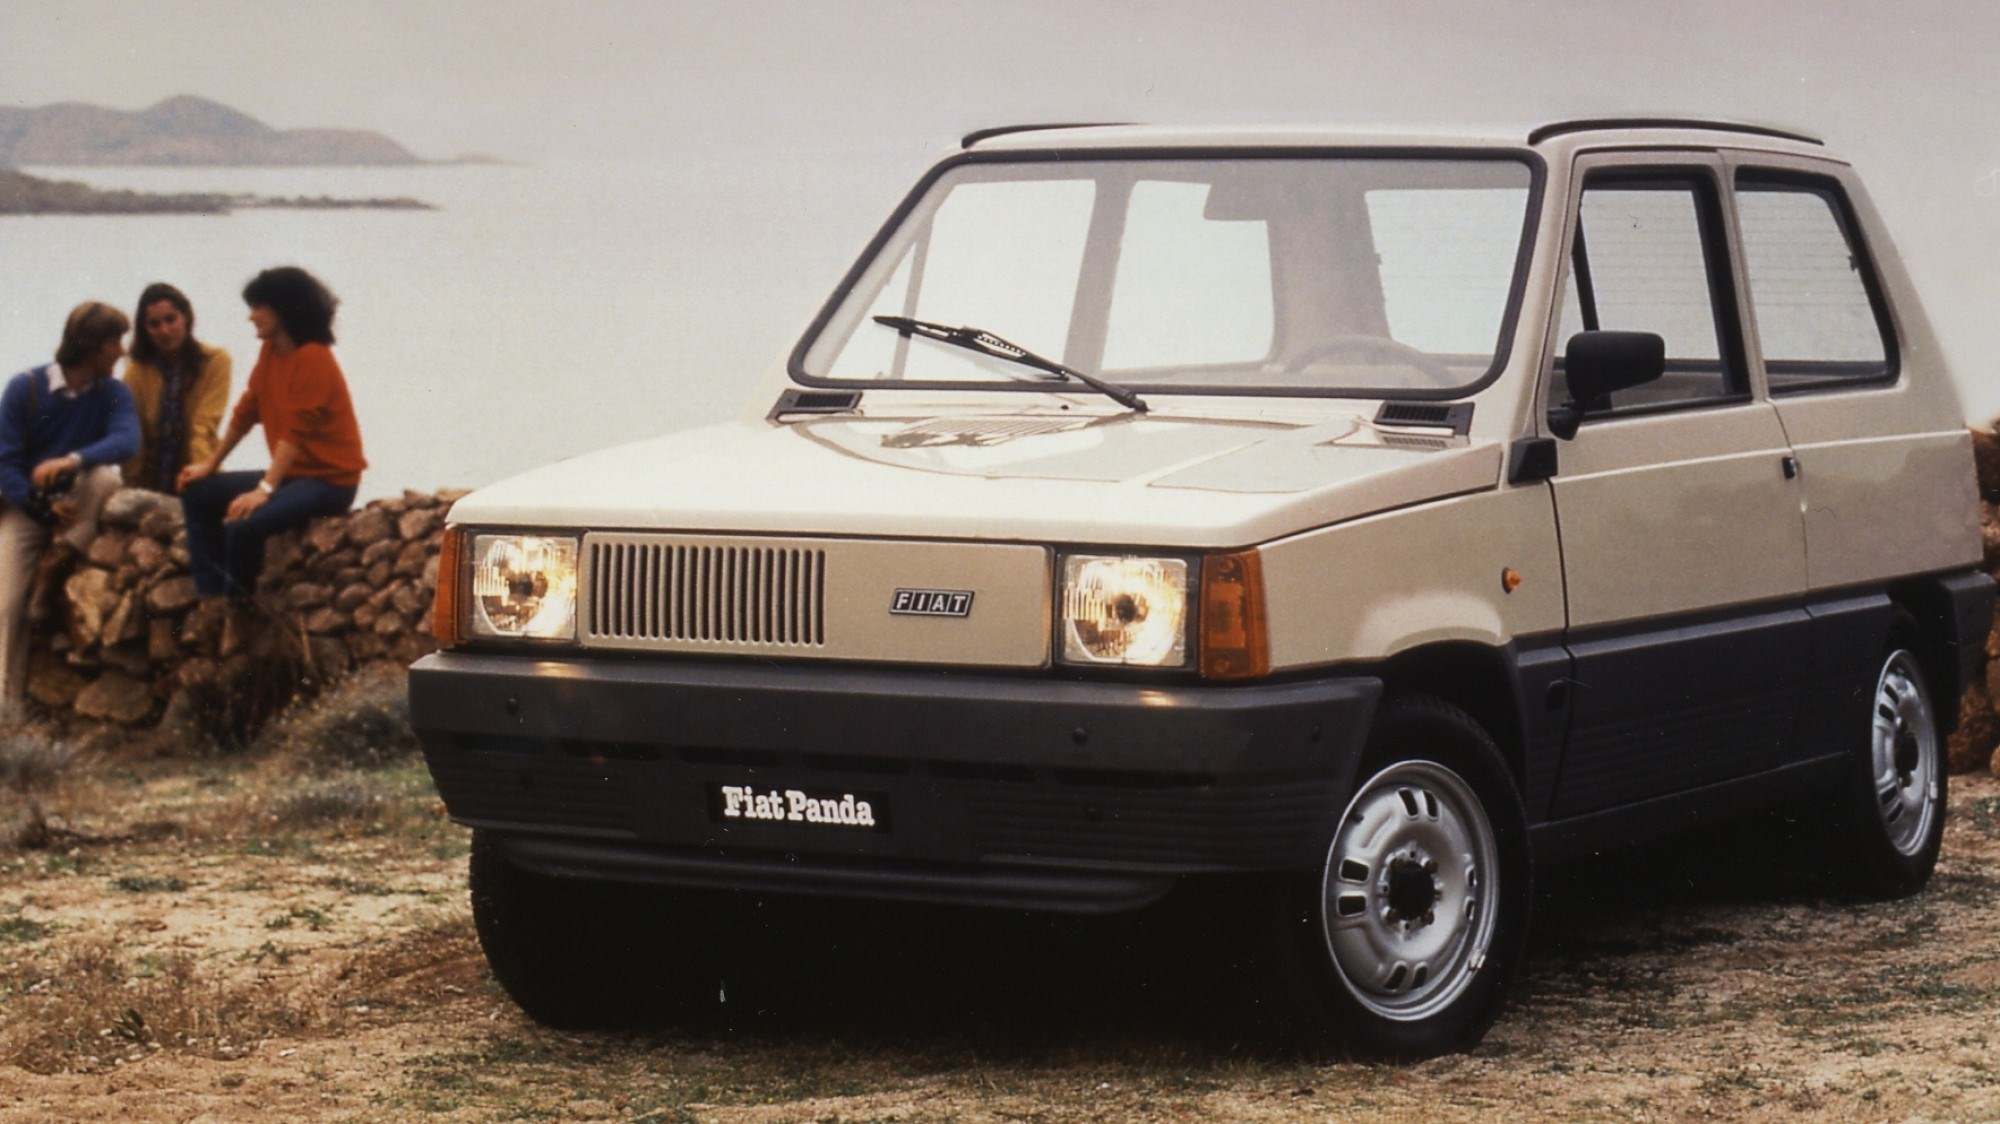
\includegraphics[scale=0.25]{pictures/dud/pic1.jpg}
\centering
\caption{Fiat Panda 141A Prima Serie}
\label{fig:Panda_esterni}
\end{figure}

\begin{figure}[H]
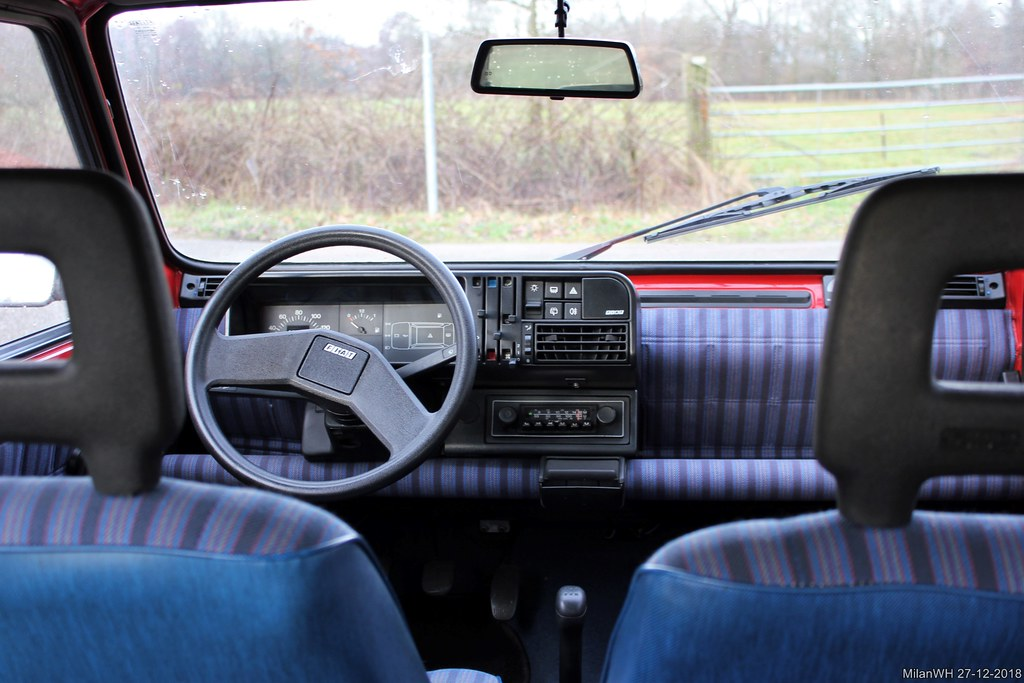
\includegraphics[scale=0.35]{pictures/dud/pic2.jpg}
\centering
\caption{Fiat Panda 141A Seconda Serie - doskonałe i praktyczne wnętrzne}
\label{fig:Panda_interni}
\end{figure}
\newpage
\textbf{FIAT PANDA - La Grande Utilitaria}\\
Swoją praktycznością Fiat Panda pokonywał wszystkie samochody w kategorii samochodów miejskich. Bagażnik miał wymiary \(54\;cm\;x\;126\;cm\;x\;40\;cm\), co daje minimalną pojemność równą: \[5.4 * 12.6 * 4 \approx 272\;dm^3\]
Jednak po złożeniu siedzeń pojemność ta wzrastała do \(632\;dm^3\), a całkowita łączna pojemność bagażnika (aż do sufitu) wynosi \(984\;dm^3\). Wynik ten do dziś budzi podziw, ale na tym nie koniec praktyczności. Siedzenia można ustawić w siedmiu różnych pozycjach, auto można wykorzystać do przeprowadzki (co sam uczyniłem przenosząc się do Krakowa, zmieściłem wszystkie swoje rzeczy!) albo do spania (tylko pierwsza seria, potem wprowadzono obowiązkowe pasy z tyłu). Przykładowe dwie pozycje foteli przedstawiono na ilustracji \ref{fig:Panda_sedile_posteriore}.

\begin{figure}[H]
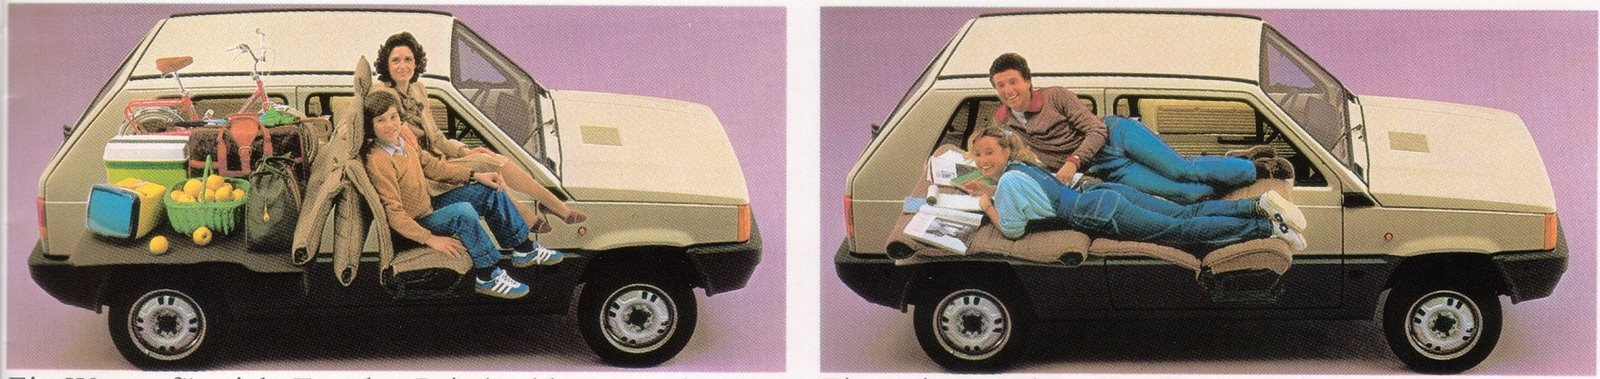
\includegraphics[scale=0.25]{pictures/dud/pic3.jpg}
\centering
\caption{Fiat Panda 141A Prima Serie - wybrane dwa ustawienia foteli}
\label{fig:Panda_sedile_posteriore}
\end{figure}
